\section{Ingestion}
Bei der Entwicklung der Ingestion wird das Laden der Daten und die Architektur der Anwendung betrachtet.
Es wird eine Datenmodell, in dem die Informationen zu den Datenquellen gespeichert werden, der Ablauf der verschiedenen Ingestion-Prozesse und die Kommunikation zwischen den einzelnen Mircoservices entwickelt.

\subsection{Server Architektur}
\label{sec:arch}

\begin{figure}
    \centering
    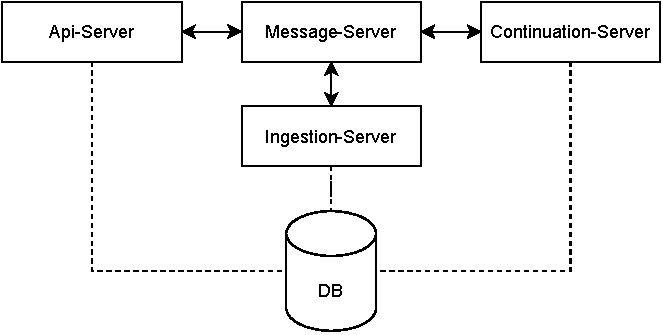
\includegraphics{Grafiken/ingestion-arch.pdf}
    \caption{Architektur der Ingestion Komponenten}
    \label{fig:ingestion_arch}
\end{figure}

Für die Umsetzung der Mircoservice-Architektur wird die Ingestion in Komponenten aufgeteilt, die \fref{fig:ingestion_arch} zu sehen sind.
Es gibt drei Services, die für die Ingestion spezifischen Aufgaben zuständig sind, eine Datenbank, in der die Informationen über Datenquellen gespeichert werden und einen Service, der für die Kommunikation verantwortlich ist.
Der \textbf{Api-Server} bietet einen REST-Schnittstelle, über die man mit der Ingestion interagieren kann.
Hier werden die Endpunkte aus \fref{tab:enpoints} benötigt, die die Schnittstellen zur Verwaltung von Datenquellen und das Ausführen von Ingestions bereitstellen.
Außerdem ist er dafür zuständig, die empfangenen Informationen über Datenquellen in der Datenbank zu verwalten.
der \textbf{Continuation-Server} überprüft regelmäßig alle kontinuierlichen Datenquellen, ob diese eine Zeitsteuerung haben und aktuell ausgeführt werden sollten.
Der \textbf{Ingestion-Server} ist die Anwendung, die die eigentliche Ingestion ausführt.
Dafür wartet dieser auf eine Aufforderung durch entweder den Api- oder den Continuation-Server.

\begin{table}[!ht]
    \centering
    \begin{tabular}{| l | l | p{3in} |}
        \hline
        Pfad                                        & HTTP-Methode  & Beschreibung \\
        \hline \hline
        /datasources                                & GET           & Liefert alle im System gespeicherten Datenquellen \\
        \hline
        /datasources/\textless id\textgreater       & GET           & Liefert die Datenquelle mit der im Pfad übergebenen Id \\
        \hline
        /datasources                                & POST          & Erstellt eine neue Datenquelle \\
        \hline
        /datasources/\textless id\textgreater       & PUT           & Bearbeitet die Daten Datenquelle mit der im Pfad übergebenen Id \\
        \hline
        /datasources/\textless id\textgreater/run   & GET           & Startet eine Ingestion der Datenquelle mit der im Pfad übergebenen Id \\
        \hline
    \end{tabular}
    \caption{Endpunkte des Api-Servers}
    \label{tab:enpoints}
\end{table}

\subsection{Plugins}
Da bei manchen Ingestions nicht immer ein festgelegtes Vorgehen ausreicht, um die Daten aus bestimmten Datenqellen zu laden, muss ein System entwickelt werden, wie möglichst ohne großen Aufwand die Inegstion erweitert werden kann.
Beispiele für solche Fälle sind die Verarbeitung von Datenströmen oder die Ingestion von Daten aus APIs, die nicht generallisiert werden können.
Als Lösung für das Problem, können Plugins der Datenquelle hinzugefügt werden. 
Diese Plugins sollen Logik enthalten, die an verschiedenen Stellen der Ingestion ausgeführt werden sollen.
Aktuell sind diese Stellen das Laden der Daten, nach dem Laden der Daten und die Stream-Verarbeitung.
Dabei ist zu beachten, dass Plugins, die das Laden der Daten abhandeln, das Standardverhalten des Ingestion-Servers überschreiben und das Stream-Verarbeitung nur mit Plugins möglich ist.
Damit es nicht zu Konflikten bei Abhängigkeiten der Plugins gibt, muss der Ingestion-Server eine Mechanik implementieren, bei der die Abhängigkeiten der Plugins für jede Datenquelle dynamisch gealden werden.

\subsection{Datenquellen}
Eine letzte Vorüberlegung für die Ingestion ist, welche Informationen erfasst werden müssen, um eine generische Ingestion zu ermöglichen.
Da es keine klaren Parameter wie zum Beispiel Datenbanknamen oder IP-Adressen gibt, die bei allen Quellen gleich sind, orientiert sich die Eingabe an der Funktionsweise von \textit{Pyspark / Apache Spark}.
Um festzulegen, woher Daten gelesen werden sollen, kann man beim erstellen einer \verb|SparkSession| einmal das Format der zu lesenden Daten angeben.
Außerdem bietet die \verb|SparkSession| die Funktion Maven-Abhängigkeiten hinzuzufügen, die Unterstützung für verschiedene Formate bringen.
Bei den meisten Formaten müssen zusätzlich noch Optionen gesetzt werden, die zum Beispiel Verbindungsparameter oder Lesemodus enthalten.
Diese Optionen sind eine Sammlung von Schlüssel-Wert-Paaren.
Eine Ausnahme besteht hierbei bei der Optionen, für die Quelledateien bei Datei-Ingestions, da diese automatisch durch die Anwendung gesetzt wird.
Daraus lassen sich bereits drei Felder ableiten, die in einem Datenmodell für die Datenquellen enthalten sein müssen: Format, Pakete und Optionen.

Neben den \textit{Spark}-spezifischen Feldern soll die Datenquelle auch die anwendungsspezifischen Informationen enhalten.
Dazu gehören Informationen über den Typ der Ingestion (siehe \ref{fig:ingestion_types}), Zeitpunkt der Erstellung und Aktualisierung, Plugins und Quelldateien und die mögliche Zeitsteuerung der Inegstions.
